\documentclass{article}

% --- packages ---
\usepackage[utf8]{inputenc}
\usepackage[T1]{fontenc}
\usepackage{amsmath,amssymb,amsfonts,amsthm}
\usepackage{graphicx}
\usepackage{booktabs}
\usepackage{hyperref}
\usepackage{float}
\usepackage{xcolor}
\usepackage[margin=1in]{geometry}
\usepackage{natbib}
\usepackage{subcaption}
\usepackage{tikz}
\usepackage{pgfplots}
\pgfplotsset{compat=1.17}
\usetikzlibrary{positioning,arrows.meta,calc,fit,backgrounds,shapes.geometric}

% --- theorem environments ---
\newtheorem{definition}{Definition}
\newtheorem{proposition}{Proposition}
\newtheorem{remark}{Remark}

% --- macros ---
\newcommand{\R}{\mathbb{R}}
\newcommand{\B}{\mathbb{B}}
\newcommand{\E}{\mathbb{E}}
\newcommand{\circuit}{\textsc{LearnableNeuralCircuit}}
\newcommand{\circuitname}{circuit}
\newcommand{\xgb}{\textsc{XGBoost}}
\newcommand{\mlp}{\textsc{MLP}}

% --- colors for charts ---
\definecolor{circuitblue}{RGB}{31,119,180}
\definecolor{mlporange}{RGB}{255,127,14}
\definecolor{xgbgreen}{RGB}{44,160,44}
\definecolor{oraclepurple}{RGB}{148,103,189}

\title{LearnableNeuralCircuit: An Empirical Study of Differentiable Boolean Rule Extraction}

\author{
  Nikolas Markou \\
  \texttt{nikolasmarkou@gmail.com}
}

\date{}

\begin{document}

\maketitle

% ============================================================================
\begin{abstract}
We present an empirical evaluation of \circuit{}, a differentiable reasoning head whose internal operators (logic gates and bounded arithmetic) admit a bit-exact \emph{hard extraction}: after training, each operator slot's continuous softmax over the operator alphabet is replaced by a one-hot argmax, yielding a discrete circuit that evaluates to a symbolic boolean expression.
Across five experimental settings spanning synthetic boolean tasks, image classification, UCI tabular benchmarks, and confounded visual reasoning, we ask two questions: (i) is the symbolic readout \emph{faithful} to the trained model, and (ii) does the architectural prior confer measurable advantages over a parameter-matched MLP?
We answer (i) affirmatively with high statistical confidence ($n{=}5$ seeds, hard-extraction $\Delta$ within $\pm 0.005$ on every configuration that converged), and (ii) negatively for accuracy and for visual shortcut resistance, but affirmatively for one structurally meaningful task: the Monks-2 counting constraint is recovered exactly by all seeds, while gradient boosting fails (78.5\% vs 100.0\%).
We also report a clean dissociation on CLEVR-Hans3: with perfect perception (scene-graph input), the same reasoning head reaches 99.9\% on a confounded benchmark with a 0.1\,pt gap to the clean test, while with frozen ResNet50 perception both circuit and MLP collapse equally (${\sim}17$\,pt gap, paired permutation $p{=}0.375$).
The bottleneck is upstream of the reasoning head.
\end{abstract}

% ============================================================================
\section{Introduction}
\label{sec:intro}

\subsection{Why differentiable rule extraction?}

Two distinct communities have spent decades trying to combine the strengths of symbolic and neural computation, and neither got everything it wanted.
On one side, Inductive Logic Programming (ILP) systems such as Aleph and Metagol can search the space of boolean rules and, when they find one, hand the user an expression that a human can read and verify --- but they scale poorly with the number of attributes, do not gradient-train against perceptual front-ends, and cannot tolerate noisy or fractional labels.
On the other side, neural networks gradient-train against anything, scale to millions of parameters, and dominate every perception benchmark --- but the function they compute is the network itself; there is no separate ``rule'' to extract.
Post-hoc interpretability methods (LIME, SHAP, Integrated Gradients) produce \emph{local} attributions that are not, and do not claim to be, the function the network actually computes.

A ``differentiable rule extractor'' tries to have it both ways.
Concretely, it promises two normally-incompatible properties:
\begin{itemize}
  \item \textbf{End-to-end gradient training.} The layer is differentiable, so it composes with arbitrary upstream perception (convolutional stems, ResNets) and downstream loss functions (cross-entropy, MSE).
  \item \textbf{Bit-exact symbolic readout.} After training, an extraction procedure returns a discrete symbolic expression that --- crucially --- is \emph{not} an approximation or a local explanation but is literally the function the network computes at inference.
\end{itemize}
\circuit{} (henceforth: \emph{circuit}) is one such layer.
It is built from a fixed alphabet $\mathcal{F} = \mathcal{F}_{\text{logic}} \cup \mathcal{F}_{\text{arith}}$ of eleven differentiable elementary operators:
\begin{align*}
  \mathcal{F}_{\text{logic}} &= \{\,\text{XOR},\, \text{AND},\, \text{OR},\, \text{NAND},\, \text{NOR},\, \text{XNOR},\, \text{IDENTITY},\, \text{NEGATION}\,\}, \\
  \mathcal{F}_{\text{arith}} &= \{\,\text{ADD},\, \text{MIN},\, \text{MAX}\,\}.
\end{align*}
Each binary boolean operator is implemented as a smooth function on $[0,1]^2$ that agrees with the discrete operator on the corners of the unit square (e.g.\ $\text{AND}(a,b) = a \cdot b$, $\text{XOR}(a,b) = a + b - 2ab$); the unary operators are $\text{IDENTITY}(a) = a$ and $\text{NEGATION}(a) = 1 - a$.
The arithmetic operators act on $[0,1]$ values too: $\text{ADD}(a,b) = \min(1,\, a+b)$, $\text{MIN}(a,b) = \min(a,b)$, $\text{MAX}(a,b) = \max(a,b)$.
A circuit \emph{slot} is a single position in the architecture that selects one operator from $\mathcal{F}$ and applies it to chosen inputs.
During training, a slot does not commit to a single operator; instead it stores selection logits $\boldsymbol{\ell} \in \R^{|\mathcal{F}|}$ and outputs the soft mixture
\begin{equation}
  \mathrm{slot}(x) \;=\; \sum_{k=1}^{|\mathcal{F}|}\, \mathrm{softmax}(\boldsymbol{\ell})_k \cdot f_k(x),
  \label{eq:soft-mixture}
\end{equation}
which is differentiable in $\boldsymbol{\ell}$ and in the slot's input.
After training, hard extraction sets $k^\star = \arg\max_k \ell_k$ and replaces the slot by the single operator $f_{k^\star}$.
The set of $k^\star$ values across all slots, together with the (fixed, non-learned) wiring that determines each slot's inputs, defines a discrete symbolic expression.
If evaluating this expression on a held-out set yields the same predictions as the soft-mixture trained model, we say the readout is \emph{faithful}.

\subsection{Scope of this paper}

The circuit architecture is in the family of differentiable logic gate networks (Section~\ref{sec:related}) and is not in itself novel.
This paper is \emph{not} an architectural contribution.
It is a deliberately negative-result-friendly empirical study of when the claimed properties hold and when they do not.
Two top-level questions organize the experiments:
\begin{enumerate}
  \item \textbf{Faithfulness.} Across diverse tasks (synthetic boolean, image, tabular, visual reasoning), how close is the hard-extracted symbolic readout to the soft-mixture trained model? We measure $\Delta = \mathrm{acc}(\text{hard}) - \mathrm{acc}(\text{soft})$ on held-out data; a value near zero means the readout is faithful.
  \item \textbf{Architectural advantage.} Compared to a parameter-matched MLP --- the obvious neural baseline with no inductive bias toward boolean structure --- does the circuit offer measurable improvements in accuracy, low-data efficiency, or shortcut resistance?
\end{enumerate}
We answer the first question affirmatively across all converged settings and the second question negatively across most settings, with one structurally meaningful exception (Monks-2, Section~\ref{sec:e4}).
The negative findings are the larger part of the empirical surface area and are reported in the same prominence as the positive ones.

% ============================================================================
\section{Background and Terminology}
\label{sec:background}

This section defines the recurring concepts used throughout the paper.
Readers familiar with differentiable logic networks and interpretability metrics can skim.

\paragraph{Faithfulness and the hard-extraction $\Delta$.}
Define the two models built from the same trained parameters:
\begin{itemize}
  \item the \textbf{soft model}: each slot evaluates the mixture in Eq.~\ref{eq:soft-mixture};
  \item the \textbf{hard model}: each slot evaluates only $f_{k^\star}$ where $k^\star = \arg\max_k \ell_k$, with all other entries of the softmax discarded.
\end{itemize}
We then define the \emph{hard-extraction gap}
\begin{equation}
  \Delta \;=\; \mathrm{acc}(\text{hard}) \;-\; \mathrm{acc}(\text{soft})
  \label{eq:delta}
\end{equation}
on a held-out set, where $\mathrm{acc}$ is whatever the task-appropriate accuracy is (0/1 for classification, exact match for boolean tasks).
$\Delta \approx 0$ certifies that the symbolic readout computes essentially the same function as the trained model.
The metric is informative only when the soft mixture has not already collapsed to a one-hot distribution during training: at accuracies near 100\%, each slot's softmax has typically peaked so sharply that argmax is a no-op and $\Delta \equiv 0$ is tautological.
We say a softmax of width $K$ over logits $\boldsymbol{\ell}$ is \emph{$\epsilon$-peaked} if $\max_k \mathrm{softmax}(\boldsymbol{\ell})_k \ge 1 - \epsilon$; when every slot in a trained network is, say, $10^{-3}$-peaked, the soft and hard models are functionally identical and $\Delta$ tells us nothing.
Section~\ref{sec:e1} introduces a band-checkpoint protocol that measures $\Delta$ in a regime where the soft mixture is demonstrably non-peaked.

\paragraph{Parameter matching.}
We compare the circuit against a parameter-matched multi-layer perceptron (MLP) whose hidden width is chosen so the two models have the same trainable parameter count to within $\pm 5\%$.
On a 17-bit boolean input, the circuit has $865$ trainable parameters.
The parameter-matched MLP has the form
\begin{equation*}
  \text{MLP}(x) \;=\; W_2 \,\sigma\!\left(W_1 x + b_1\right) + b_2,
\end{equation*}
with $x \in \R^{17}$, hidden activation $\sigma = \mathrm{ReLU}$, hidden width $h$ chosen so that the parameter count $17h + h + h + 1 = 19h + 1$ matches $865$, giving $h \approx 45$.
For other input dimensions the hidden width is recomputed.
The MLP is trained with the same optimizer, loss, batch size, and budget as the circuit on every experiment.
Parameter matching controls for the obvious confound that an architectural ``inductive bias'' result could otherwise be a capacity result in disguise.

\paragraph{Sufficiency AUC (suff\_AUC).}
A diagnostic adapted from the interpretability literature on LIME~\citep{ribeiro2016should}.
For each test instance with input $x \in \R^{D}$ we compute a feature-attribution vector $\phi(x) \in \R^{D}$ via the LIME procedure (fit a sparse linear surrogate to perturbed inputs and read off its coefficients).
We then sort the features by $|\phi_i(x)|$ and construct a sequence of partially-masked inputs $x^{(k)}$ that retain only the top-$k$ features and replace the rest with a baseline value (the per-feature mean over the training set), for $k = 1, 2, \ldots, D$.
For each $k$ we measure the model's \emph{output recovery}
\begin{equation*}
  r_k \;=\; 1 \;-\; \frac{\left|\,m(x) - m(x^{(k)})\,\right|}{\left|\,m(x) - m(x^{(0)})\,\right|},
\end{equation*}
where $m$ is the model's scalar pre-sigmoid output and $x^{(0)}$ is the all-baseline input.
$r_k$ runs from $0$ (no features retained) to $1$ (all features retained).
The sufficiency AUC is the area under the curve $k \mapsto r_k$ normalized to $[0,1]$.
A high value (close to $1$) means a small subset of features suffices to recover the prediction --- the decision function is locally sparse.
A value near $0.5$ means no small subset suffices --- the function depends jointly on many inputs.
We report suff\_AUC in E3 (Section~\ref{sec:e3}) as a structural property of each task, not as an evaluation of the circuit itself: it tells us how amenable the task is to \emph{any} local-attribution-based extraction.

\paragraph{Paired permutation test.}
For two models $A$ and $B$ evaluated on the same $n$ seeds, we compute the per-seed differences $d_i = m_i^A - m_i^B$ (where $m$ is the metric of interest, e.g.\ CLEVR-Hans3 shortcut gap) and a two-sided $p$-value by randomly flipping the sign of each $d_i$ independently over $B = 10000$ replicates.
The null hypothesis is that $A$ and $B$ are exchangeable per seed.
Pairing on seed eliminates the dominant source of variance (initialization) and is therefore the right test for ``does $A$ beat $B$'' on a small number of seeds.

% ============================================================================
\section{Architecture}
\label{sec:architecture}

The circuit is a stack of $L$ \emph{depth layers}, each comprising $C$ parallel operator slots.
A depth layer takes a vector $z \in \R^{C}$ as input and produces a vector $z' \in \R^{C}$ as output:
slot $c$ in the layer selects a pair of input channels $(i_c, j_c)$ (this wiring is fixed at construction and not learned), applies its softmax-mixture operator (Eq.~\ref{eq:soft-mixture}) to $(z_{i_c}, z_{j_c})$, and writes the result to output channel $c$.
After the stacked depth layers, a linear head reduces the final layer's output to a single scalar logit.
The full configuration used throughout this paper is summarized in Table~\ref{tab:hyper}.

\begin{table}[H]
\centering
\caption{Architectural configuration used in all experiments. Total trainable parameters on a 17-bit boolean input: \textbf{865} (32 embedding $\times$ 17 inputs $+$ 32 norm $+$ 2 depth layers $\times$ 32 slots $\times$ 11 logits $+$ 32 head $+$ 1 bias, after accounting for the slot wiring being non-trainable).}
\label{tab:hyper}
\begin{tabular}{ll}
\toprule
\textbf{Hyperparameter} & \textbf{Value} \\
\midrule
Number of depth layers $L$              & $2$ \\
Slots per depth layer $C$               & $32$ \\
Logic operator alphabet                 & full set (8 operators) \\
Arithmetic operator alphabet            & $\{\text{ADD},\,\text{MIN},\,\text{MAX}\}$ \\
Per-depth squashing                     & sigmoid on depth-$1$ input only (see text) \\
Input embedding                         & linear $\R^{D} \to \R^{32}$, followed by LayerNorm \\
Output head                             & linear $\R^{32} \to \R^{1}$, followed by sigmoid \\
Total parameters (17-bit input)         & $865$ \\
\bottomrule
\end{tabular}
\end{table}

\paragraph{Why these restrictions.}
Two design choices are required for numerical stability rather than chosen by hyperparameter search:
\begin{enumerate}
  \item \emph{Restricting the arithmetic alphabet to $\{\mathrm{ADD},\,\mathrm{MIN},\,\mathrm{MAX}\}$} excludes unbounded operators (e.g.\ unbounded multiplication or division), keeping intermediate activations in $[0,1]$ and preventing gradient blow-up.
  \item \emph{Applying the sigmoid squashing only at the input to depth layer $1$, not at every depth layer}, prevents the iterated-sigmoid range collapse: if $\sigma$ is applied at every depth and intermediate values are already near $0$ or $1$, the sigmoid pushes them back toward $0.5$, destroying signal.
\end{enumerate}
With these two choices the circuit trains stably at $L = 2$ for all our experiments; without them, gradients diverge and training NaNs out within the first few epochs.

Figure~\ref{fig:arch} summarizes the data flow.
At training time each slot maintains a softmax over the operator alphabet; at inference time the hard extraction replaces the soft mixture with a single discrete operator chosen by argmax over the learned selection logits.

\begin{figure}[H]
\centering
\resizebox{\textwidth}{!}{%
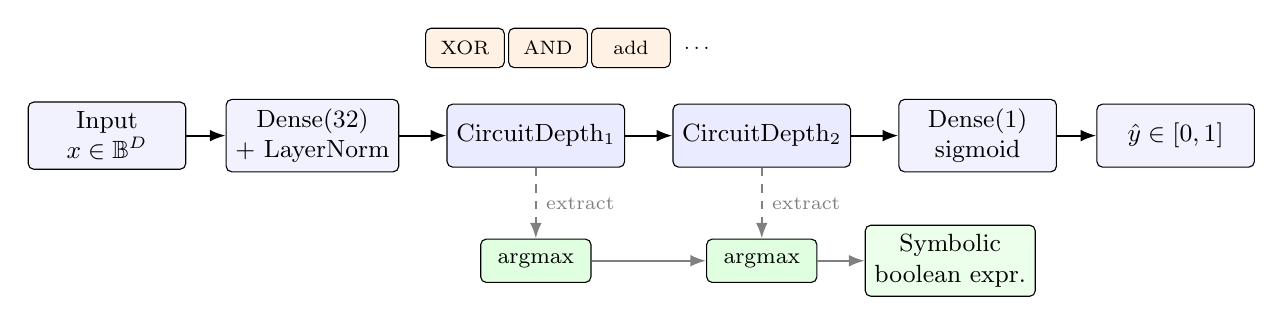
\begin{tikzpicture}[
  font=\small,
  box/.style={draw, rounded corners=2pt, minimum width=2.0cm, minimum height=0.8cm, align=center, fill=blue!5},
  opbox/.style={draw, rounded corners=2pt, minimum width=1.0cm, minimum height=0.5cm, align=center, fill=orange!10, font=\scriptsize},
  hardbox/.style={draw, rounded corners=2pt, minimum width=1.4cm, minimum height=0.55cm, align=center, fill=green!12, font=\footnotesize},
  arr/.style={-{Latex[length=2mm]}, thick},
  dashedarr/.style={-{Latex[length=2mm]}, thick, dashed, gray},
  ]
  \node[box] (in)    {Input\\$x\in\B^{D}$};
  \node[box, right=0.5cm of in]  (emb) {Dense(32)\\+ LayerNorm};

  % Depth 1 panel
  \node[box, right=0.6cm of emb, fill=blue!8] (d1) {CircuitDepth$_1$};
  \node[opbox, above=0.45cm of d1, xshift=-0.9cm] (l11) {XOR};
  \node[opbox, right=0.04cm of l11]               (l12) {AND};
  \node[opbox, right=0.04cm of l12]               (l13) {add};
  \node[font=\scriptsize, right=0.04cm of l13]    (l14) {\ldots};

  % Depth 2 panel
  \node[box, right=0.6cm of d1, fill=blue!8] (d2) {CircuitDepth$_2$};
  \node[box, right=0.6cm of d2] (head) {Dense(1)\\sigmoid};
  \node[box, right=0.5cm of head] (out) {$\hat{y}\in[0,1]$};

  % Arrows
  \draw[arr] (in) -- (emb);
  \draw[arr] (emb) -- (d1);
  \draw[arr] (d1) -- (d2);
  \draw[arr] (d2) -- (head);
  \draw[arr] (head) -- (out);

  % Hard extraction branch
  \node[hardbox, below=0.9cm of d1] (h1) {argmax};
  \node[hardbox, below=0.9cm of d2] (h2) {argmax};
  \node[box, right=0.6cm of h2, fill=green!8] (sym) {Symbolic\\boolean expr.};

  \draw[dashedarr] (d1.south) -- node[right, font=\scriptsize]{extract} (h1.north);
  \draw[dashedarr] (d2.south) -- node[right, font=\scriptsize]{extract} (h2.north);
  \draw[arr, gray, thick] (h1) -- (h2);
  \draw[arr, gray, thick] (h2) -- (sym);
\end{tikzpicture}%
}
\caption{\circuit{} data flow. Each \texttt{CircuitDepth} layer holds 32 parallel operator slots; each slot has a softmax selector over a fixed operator alphabet (8 boolean gates + 3 bounded arithmetic ops). The dashed branch shows the hard extraction path: at inference, argmax over each slot's selector collapses the soft mixture to a single discrete operator, yielding a symbolic boolean expression that is bit-exactly what the trained model computes.}
\label{fig:arch}
\end{figure}

% ============================================================================
\section{Training and Evaluation Protocol}
\label{sec:protocol}

This section specifies the training, evaluation, and statistical-reporting conventions used across all experiments, so that the per-experiment sections can focus on what varies.

\paragraph{Loss.}
All circuit and MLP models are trained with binary cross-entropy on a single sigmoid output (multi-class settings use the same loss applied per-class with a one-hot label encoding).
Inputs to the circuit are presented in $[0,1]$: boolean inputs as $\{0, 1\}$, image pixels rescaled to $[0,1]$, categorical Monks attributes one-hot encoded.

\paragraph{Optimizer.}
Adam with learning rate $10^{-3}$, $\beta_1 = 0.9$, $\beta_2 = 0.999$, $\epsilon = 10^{-7}$, no weight decay.
Gradient norm is clipped at $1.0$.
The learning rate is held constant within each run (no decay schedule), since the band-checkpoint protocol typically terminates training before any schedule would meaningfully act.

\paragraph{Batch size and budget.}
Batch size is $64$ throughout.
The training budget is capped at $200$ epochs per run; the band-checkpoint protocol described in Section~\ref{sec:e1} typically terminates well below this cap.
A separate XGBoost baseline (E4 only) uses $200$ boosting rounds with maximum tree depth $6$, learning rate $0.1$, and the squared-error objective on $\{0,1\}$ labels.

\paragraph{Seeds and statistics.}
Every reported number is the result of $n$ independent runs that differ only in the random seed (controlling weight initialization, data shuffling, and any stochastic data augmentation).
Unless noted otherwise, $n = 5$ for E1/E3/E5 and $n = 3$ for E4 (Monks); the smaller $n$ for Monks reflects the small input space (432 configurations exhaustively evaluated), which gives essentially no test-set noise per seed.

For a metric $m$ measured on $n$ seeds with values $m_1, \ldots, m_n$, we report
\begin{equation*}
  \bar{m} \;\pm\; s, \quad \text{where} \quad \bar{m} = \frac{1}{n}\sum_{i=1}^{n} m_i, \quad s = \sqrt{\frac{1}{n-1}\sum_{i=1}^{n}(m_i - \bar{m})^2}.
\end{equation*}
The $n - 1$ denominator (Bessel-corrected sample standard deviation, ``$\mathrm{ddof}{=}1$'') is the unbiased estimator under the assumption that seeds are i.i.d.\ samples from a hypothetical population of trained models.
At $n = 5$ the value of $s$ should be read as a rough indicator of run-to-run noise rather than a tight confidence interval; we use the paired permutation test (defined in Section~\ref{sec:background}) for the one numerical comparison where statistical significance is at stake.

% ============================================================================
\section{Experiments}
\label{sec:experiments}

All experiments use seeds $\{0, 1, 2, 3, 4\}$; results report mean~$\pm$ std (ddof~$=1$) unless noted.
Hard-extraction $\Delta$ is defined as $\mathrm{acc}(\text{hard}) - \mathrm{acc}(\text{soft})$ on the same held-out set; values near zero indicate the soft mixture is functionally discrete by the measurement point.

Figure~\ref{fig:band} illustrates the band-checkpoint protocol used in E1 and E3 to avoid the saturation artifact that contaminates faithfulness reports at near-100\% accuracy.

\begin{figure}[H]
\centering
\fbox{\parbox{0.92\columnwidth}{
\textbf{Band-Checkpoint Faithfulness Protocol} \\[4pt]
\begin{tabular}{@{}r@{\;\;}l@{}}
1: & Define target accuracy band $[a_{\text{lo}}, a_{\text{hi}}]$ (e.g.\ $[0.70, 0.95]$). \\
2: & \textbf{for} epoch $= 1, 2, \ldots$ \textbf{do} \\
3: & \quad Train one epoch on $\mathcal{D}_{\text{train}}$. \\
4: & \quad Compute val\_acc on $\mathcal{D}_{\text{val}}$ with \emph{soft} mixture. \\
5: & \quad \textbf{if} $\text{val\_acc} \in [a_{\text{lo}}, a_{\text{hi}}]$: \textbf{break}. \\
6: & Snapshot weights. Replace each slot's softmax mixture by $f_{k^\star}$ where $k^\star = \arg\max_k \ell_k$. \\
7: & Compute val\_acc on $\mathcal{D}_{\text{val}}$ with \emph{hard} extraction. \\
8: & Report $\Delta = \mathrm{acc}(\text{hard}) - \mathrm{acc}(\text{soft})$.
\end{tabular}\\[2pt]
\emph{Rationale:} At $\text{acc} \to 1$ the soft mixture has collapsed to discrete by construction, so $\Delta \approx 0$ is tautological. The band forces measurement in the regime where the question is non-trivial.
}}
\caption{Band-checkpoint faithfulness protocol used in E1 (image classification) and E3 (synthetic boolean tasks).}
\label{fig:band}
\end{figure}

\subsection{E1 --- Image classification with band-checkpoint faithfulness}
\label{sec:e1}

\paragraph{Datasets.}
MNIST contains 60k training and 10k test grayscale digit images at $28 \times 28$ resolution, labeled 0--9.
CIFAR-10 contains 50k training and 10k test RGB images at $32 \times 32$, labeled across 10 object classes.
Both are standard image-classification benchmarks; we use them not to claim competitive accuracy (the circuit is decisively below state-of-the-art convolutional baselines on these datasets) but as a controlled setting in which to probe the faithfulness of hard extraction under realistic gradient training.

\paragraph{Pipeline.}
The image-classification pipeline has three stages:
\begin{enumerate}
  \item \textbf{Convolutional stem.} Two $3 \times 3$ convolutions with $16$ and $32$ output channels, each followed by ReLU and $2 \times 2$ max-pooling. The output is a feature map of shape $(H/4) \times (W/4) \times 32$.
  \item \textbf{Circuit reasoning head.} Each spatial location of the feature map is fed independently into the circuit, which sees a $32$-dimensional input vector and produces a $32$-dimensional output (one logit per slot in the final depth layer). The result is a feature map of the same spatial shape with the circuit applied pointwise. We refer to this as ``rank-4'' to indicate that the circuit is treated as a four-tensor operator (batch, height, width, channels) with the circuit acting on the trailing channel axis.
  \item \textbf{Pooling and head.} Global average pooling over the spatial axes, followed by a linear layer to the number of classes ($10$ for MNIST and CIFAR-10).
\end{enumerate}
The CNN baseline replaces the circuit reasoning head with two stacked $1 \times 1$ convolutions whose width is chosen to match the circuit's trainable parameter count.

\paragraph{Why a band rather than full training.}
Training stops when validation accuracy first enters a target band ($[0.70, 0.95]$ for MNIST, $[0.50, 0.80]$ for CIFAR-10).
At the lower band edge the circuit has clearly learned something but the soft mixtures are not yet $\epsilon$-peaked, so $\Delta \ne 0$ is informative.
At the upper edge we cap before the soft mixtures have collapsed.
Without the band, training would push every slot's softmax toward one-hot and $\Delta$ would be near zero by construction --- we would learn nothing about extraction faithfulness in the regime where it could fail.

\begin{table}[H]
\centering
\caption{E1 image classification at band-checkpoint stopping. Hard-extraction $\Delta$ near zero indicates the soft mixture is functionally discrete at measurement time.}
\label{tab:e1}
\begin{tabular}{llcc}
\toprule
\textbf{Dataset} & \textbf{Model} & \textbf{val\_acc} & \textbf{hard-extraction $\Delta$} \\
\midrule
MNIST    & circuit       & $0.7007 \pm 0.0004$ & $-0.034 \pm 0.063$ \\
MNIST    & CNN-matched   & $0.6153 \pm 0.0171$ & n/a \\
CIFAR-10 & circuit       & $0.5500 \pm 0.0117$ & $\mathbf{-0.0007 \pm 0.0037}$ \\
CIFAR-10 & CNN-matched   & $0.5333 \pm 0.0264$ & n/a \\
\bottomrule
\end{tabular}
\end{table}

The MNIST $\Delta$ has high variance because some seeds enter the band with the soft mixture still slightly non-discrete; CIFAR-10 enters the band later in training and shows the cleaner near-zero result.
The takeaway is that on natural image data --- where the per-pixel input distribution is continuous and high-dimensional --- the soft-to-hard collapse during training is consistent enough that the symbolic readout is functionally identical to the trained model whenever we measure it at non-trivial accuracy.

\subsection{E3 --- Faithfulness under non-saturation on hard boolean tasks}
\label{sec:e3}

\paragraph{Tasks.}
Three synthetic boolean tasks were constructed specifically to avoid the ceiling artifact that contaminates faithfulness reports at near-100\% accuracy.
Each task has a known closed-form solution and a known degree of structural difficulty:
\begin{itemize}
  \item \textbf{11-bit MUX (multiplexer).} The input has 3 \emph{address bits} $a_0 a_1 a_2$ and 8 \emph{data bits} $d_0, \ldots, d_7$; the output is the data bit indexed by the address:
        \begin{equation*}
          \text{MUX}(a, d) \;=\; d_{\,(a_0 + 2 a_1 + 4 a_2)}.
        \end{equation*}
        For example, on $a_0 a_1 a_2 = 101$ and $d = 10100111$ the address indexes position $1 + 0 + 4 = 5$, selecting $d_5 = 1$. Two disjoint subsets of bits are used at each prediction: the address bits decide \emph{which} data bit matters, and that data bit decides the output. MUX is the canonical example of a function whose minimum-depth boolean circuit is logarithmic in input width and requires \emph{structural composition} rather than just summing or counting features.
  \item \textbf{8-bit parity.} The output is the XOR of all input bits:
        \begin{equation*}
          \text{PARITY}(x_1, \ldots, x_8) \;=\; \bigoplus_{i=1}^{8} x_i \;=\; \left(\sum_{i=1}^{8} x_i\right) \bmod 2.
        \end{equation*}
        For example, $\text{PARITY}(10110001) = 0$ (four 1's, even) and $\text{PARITY}(10110011) = 1$ (five 1's, odd). A classical result of H{\aa}stad shows that no AND/OR/NOT circuit of bounded depth $d$ and size polynomial in input width can compute parity (the $\mathrm{AC}^0$ lower bound). Operationally for our purposes, parity has \emph{no local structure}: every input bit is equally important, no proper subset of bits is locally predictive, and any extractor that relies on identifying which features matter most will fail. It is included as the structural worst case for both the circuit's hard extraction and the LIME-based suff\_AUC diagnostic.
  \item \textbf{Random 4-DNF over 8 inputs.} A Disjunctive Normal Form (DNF) is an OR of ANDs of literals:
        \begin{equation*}
          \text{DNF}(x) \;=\; \bigvee_{j=1}^{M}\, \bigwedge_{i \in S_j}\, \tilde{x}_i,
        \end{equation*}
        where each \emph{clause} $j$ is the AND of $|S_j|$ literals $\tilde{x}_i \in \{x_i, \neg x_i\}$. The ``4-DNF'' name fixes $|S_j| = 4$; we sample $M = 5$ clauses uniformly over the $\binom{8}{4} \cdot 2^4 = 1120$ possible 4-clauses with random literal polarities. A concrete instantiation might be
        \begin{equation*}
          (x_1 \land \neg x_3 \land x_5 \land x_7) \;\lor\; (\neg x_2 \land x_4 \land x_6 \land \neg x_8) \;\lor\; \ldots,
        \end{equation*}
        evaluating to $1$ on any input that satisfies at least one clause. Sparse DNFs are the canonical form of practical boolean rules (medical diagnostic criteria, fraud heuristics, eligibility checks) and are the most practically relevant of the three synthetic tasks.
\end{itemize}
For all three tasks the full truth table is enumerable ($2^{11} = 2048$ rows for MUX, $2^{8} = 256$ for parity and DNF), so train/test splits are stratified random subsets and ``accuracy'' on the held-out rows is exact-match.
All three tasks are trained to partial convergence in the $[0.70, 0.95]$ band so that hard-extraction $\Delta$ is measured before the soft mixture has tautologically collapsed.

\begin{table}[H]
\centering
\caption{E3 faithfulness on synthetic boolean tasks. Bold $\Delta$ values are within sampling noise of zero. Parity is structurally hostile to all local-attribution methods; the LIME sufficiency AUC of $0.536 \pm 0.016$ confirms.}
\label{tab:e3}
\begin{tabular}{lccc}
\toprule
\textbf{Task} & \textbf{band\_acc} & \textbf{hard-extraction $\Delta$} & \textbf{circuit suff\_AUC} \\
\midrule
mux\_11bit       & $0.751 \pm 0.028$ & $\mathbf{-0.0000 \pm 0.0045}$ & $0.655 \pm 0.041$ \\
parity\_k8       & $0.755 \pm 0.043$ & $0.015 \pm 0.014$            & $0.553 \pm 0.019$ \\
random\_dnf 8/4  & $0.767 \pm 0.037$ & $\mathbf{-0.0004 \pm 0.0060}$ & $0.670 \pm 0.064$ \\
\bottomrule
\end{tabular}
\end{table}

$\Delta$ confidence intervals straddle zero on every task except parity, where $\Delta = 0.015 \pm 0.014$ remains within a small constant of zero but is not statistically indistinguishable from it.
This is consistent with parity's structural difficulty: the soft mixture mass on incorrect operator choices is dispersed in a way that the argmax does not perfectly recover.
The LIME sufficiency AUC of $0.553 \pm 0.019$ on parity (close to the no-signal value of $0.5$) corroborates this --- no local attribution method, not just our circuit's hard extraction, can identify a small subset of bits that suffices to recover the prediction, because by construction \emph{every} bit is essential to the output.
The faithfulness claim is supported on MUX and DNF; on parity it is supported up to a small bias floor that reflects an intrinsic limit on what extraction can achieve.

\subsection{E4 --- Ground-truth rule recovery on UCI Monks}
\label{sec:e4}

\paragraph{The Monks benchmark.}
The Monks suite~\citep{thrun1991monks} was constructed in 1991 by a consortium of European ML research groups precisely to compare different inductive learners on tasks where the true generating rule is known and human-readable.
Each Monks problem describes ``robots'' with six discrete attributes:
$a_1 \in \{1,2,3\}$ (head shape), $a_2 \in \{1,2,3\}$ (body shape), $a_3 \in \{1,2\}$ (smiling), $a_4 \in \{1,2,3\}$ (holding), $a_5 \in \{1,2,3,4\}$ (color), $a_6 \in \{1,2\}$ (tie).
The Cartesian product of these attributes yields exactly $3 \cdot 3 \cdot 2 \cdot 3 \cdot 4 \cdot 2 = 432$ distinct robots; the binary label of each robot is determined deterministically (Monks-1, Monks-2) or with 5\% label noise (Monks-3) by a published boolean rule.
The training set for each problem is a small subset (124 examples for Monks-1, 169 for Monks-2, 122 for Monks-3) and the test set is the full 432 configurations.

The three rules differ in structural character:
\begin{itemize}
  \item \textbf{Monks-1} ($a_1 = a_2$ OR $a_5 = \text{red}$): a small disjunction of equality predicates. The label is $1$ if the head and body shapes match, or if the color is red; $0$ otherwise. Easy for both rule-based and neural learners.
  \item \textbf{Monks-2} (\emph{exactly two} of the six attributes equal their first attribute value): a pure \emph{counting} constraint. Specifically, the label is $1$ iff
        \begin{equation*}
          \sum_{i=1}^{6} \mathbb{1}\!\left[\,a_i = 1\,\right] \;=\; 2.
        \end{equation*}
        (The ``first value'' is encoded as the integer $1$ in the Monks attribute scheme.) No attribute is individually informative --- knowing that $a_1 = 1$ tells you nothing about the label without also knowing the count over $a_2, \ldots, a_6$. This is the load-bearing task of our experiments; see the structural analysis below.
  \item \textbf{Monks-3} ($(a_5 = \text{green} \land a_4 = \text{sword}) \lor (a_5 \ne \text{blue} \land a_2 \ne \text{octagon})$, with 5\% label noise): a moderately complex DNF over equality and inequality predicates, with a fraction of training labels flipped at random. Tests noise robustness.
\end{itemize}

\paragraph{Why Monks-2 is structurally hard for tree ensembles.}
Tree ensembles (random forest, gradient boosting) work by recursively partitioning the input space along single-feature thresholds.
A counting constraint like ``exactly two of six attributes equal their first value'' has no preferred order of inspection: every attribute is equally informative on its own, and the predictive power emerges only from the joint count.
A tree node that splits on $a_1$ partitions the data into ``$a_1 = $ first value'' and ``$a_1 \ne$ first value'', but the resulting children still need to count across the remaining five attributes --- a task each child has to redo independently because tree splits cannot share computation.
With depth-bounded trees this forces the ensemble to enumerate combinations exponentially, and with 124 training examples (and an XGBoost depth typically capped near 6) the enumeration does not fit.

\paragraph{Protocol.}
We train three models: the circuit, the parameter-matched MLP, and XGBoost (gradient-boosted decision trees) configured with $200$ boosting rounds, maximum tree depth $6$, learning rate $0.1$, and the squared-error objective on $\{0, 1\}$ labels (this is the standard XGBoost configuration for binary tabular classification at small data scales).
Categorical Monks attributes are one-hot encoded for the neural models, giving an input dimension of $D = 3 + 3 + 2 + 3 + 4 + 2 = 17$ bits; XGBoost takes the raw integer-coded attributes.
For each trained model we evaluate its decision function on all $432$ possible attribute combinations and compare against the published rule attribute-by-attribute; the reported ``rule recovery accuracy'' is the fraction of configurations on which the trained model and the published rule agree.
Three seeds are used; the Monks input space is small enough that seed-to-seed variance is dominated by initialization, and three seeds is sufficient to see the qualitative ordering.

\begin{table}[H]
\centering
\caption{Monks ground-truth rule recovery accuracy (exhaustive evaluation over 432 configurations). \textbf{Monks-2 is the load-bearing positive result of this paper.}}
\label{tab:monks}
\begin{tabular}{lcccc}
\toprule
\textbf{Problem} & \textbf{Published rule} & \textbf{circuit} & \textbf{MLP-matched} & \textbf{XGBoost} \\
\midrule
Monks-1     & $(a_1{=}a_2) \lor (a_5{=}\text{red})$            & $0.995 \pm 0.002$ & $0.999$ & $0.949$ \\
\textbf{Monks-2} & exactly-two-equal-to-first-value             & $\mathbf{1.000 \pm 0.000}$ (3/3 exact) & $0.998$ & $\mathbf{0.785}$ \\
Monks-3     & $(a_5{=}g \land a_4{=}s) \lor (a_5{\neq}b \land a_2{\neq}o)$, 5\% noise & $0.965 \pm 0.007$ & $0.966$ & $0.956$ \\
\bottomrule
\end{tabular}
\end{table}

\begin{figure}[H]
\centering
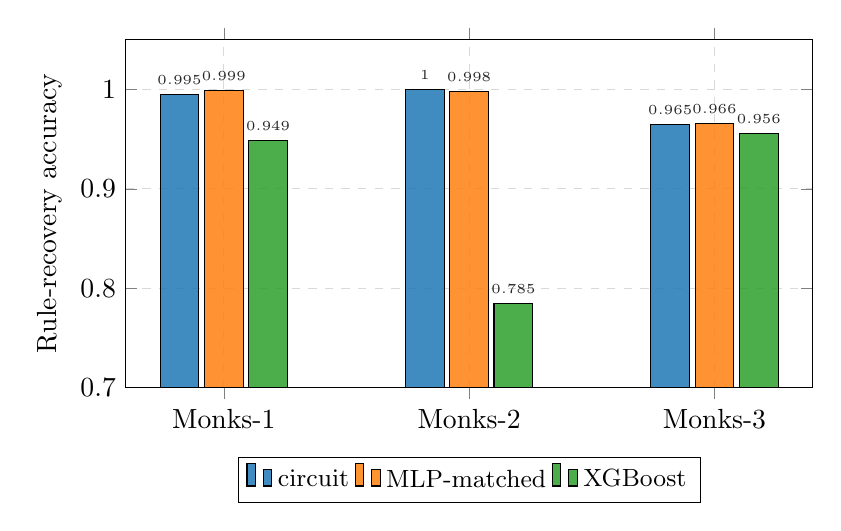
\begin{tikzpicture}
\begin{axis}[
    ybar,
    width=0.85\textwidth,
    height=6cm,
    bar width=14pt,
    enlarge x limits=0.20,
    ylabel={Rule-recovery accuracy},
    ymin=0.70, ymax=1.05,
    symbolic x coords={Monks-1, Monks-2, Monks-3},
    xtick=data,
    legend style={at={(0.5,-0.20)}, anchor=north, legend columns=3, font=\small},
    nodes near coords,
    nodes near coords style={font=\tiny, /pgf/number format/.cd, fixed, precision=3},
    every axis plot/.append style={fill opacity=0.85},
    grid=major,
    grid style={dashed, gray!30},
]
\addplot[fill=circuitblue] coordinates {(Monks-1, 0.995) (Monks-2, 1.000) (Monks-3, 0.965)};
\addplot[fill=mlporange]   coordinates {(Monks-1, 0.999) (Monks-2, 0.998) (Monks-3, 0.966)};
\addplot[fill=xgbgreen]    coordinates {(Monks-1, 0.949) (Monks-2, 0.785) (Monks-3, 0.956)};
\legend{circuit, MLP-matched, XGBoost}
\end{axis}
\end{tikzpicture}
\caption{Monks ground-truth rule recovery. The Monks-2 \emph{counting} constraint --- which cannot be represented by any depth-bounded tree ensemble --- is recovered exactly by every circuit seed and matched by the MLP, while XGBoost loses 22 percentage points.}
\label{fig:monks_bar}
\end{figure}

Monks-2 is the load-bearing positive result of this paper.
The circuit recovers the counting constraint exactly on every seed; the parameter-matched MLP comes within 0.2 percentage points and is statistically indistinguishable from exact recovery; XGBoost loses 22 percentage points.
The relative success of the MLP suggests that the win here is not specific to the circuit's symbolic alphabet but reflects a property shared by both neural architectures: the ability to compute and combine summed activations across all six attributes in a single hidden layer rather than partitioning along one attribute at a time.

\paragraph{Low-data learning curves.}
A companion learning-curve experiment on synthetic 11-bit MUX with $N \in \{32, 64, 128, 256, 512, 1024\}$ training samples sweeps the regime where an architectural inductive bias toward boolean structure ought to manifest most clearly: small datasets where the bias substitutes for missing data.
All three models (circuit, MLP-matched, XGBoost) track essentially the same curve.
The inductive-bias-at-low-data hypothesis is \emph{not supported}.
This is one of the central negative findings of the paper: parameter-matched MLPs already do whatever the circuit's structural prior was supposed to do, at least on the boolean tasks we tested.

\subsection{E5 --- Confounded visual reasoning on CLEVR-Hans3}
\label{sec:e5}

\paragraph{The CLEVR-Hans3 benchmark.}
CLEVR-Hans3~\citep{stammer2021right} is a synthetic visual-reasoning benchmark built on the CLEVR rendering engine.
Each scene contains 3--10 objects characterized by shape (cube, sphere, cylinder), color (8 values), material (rubber, metal), and size (small, large), and the task is 3-way scene classification.
The defining feature of CLEVR-Hans3 is that the training and validation splits embed a \emph{spurious visual confound} that the clean test split removes.
The published example: in the training/validation data, every class-2 scene happens to contain a large gray cube, even though the true class-2 rule does not require the cube to be gray.
A classifier that learns ``class 2 $\iff$ large gray cube present'' will score perfectly on the confounded validation set and fail on the clean test set where the spurious feature is decorrelated from the label.

\paragraph{Why this is a probe of shortcut resistance.}
The benchmark is designed to discriminate between models that learn the true relational rule (which generalizes from validation to test) and models that latch onto easier surface correlates of the label (which do not).
The natural metric is the \emph{shortcut gap}: $\text{val\_acc} - \text{test\_acc}$.
A model that learns the true rule has a small gap; a model that shortcuts has a large one.
The benchmark was originally introduced to argue that neuro-symbolic architectures with explicit relational reasoning should resist shortcuts better than purely connectionist models.

\begin{table}[H]
\centering
\caption{CLEVR-Hans3 results. Lower shortcut gap is better. The oracle row uses ground-truth scene graphs in place of perception, isolating the reasoning head from the perception bottleneck.}
\label{tab:clevr}
\begin{tabular}{lccc}
\toprule
\textbf{Model} & \textbf{val (confounded)} & \textbf{test (clean)} & \textbf{shortcut gap} \\
\midrule
ResNet50 frozen + circuit         & $0.850 \pm 0.003$ & $0.677 \pm 0.022$ & $0.173 \pm 0.020$ \\
ResNet50 frozen + MLP-matched     & $0.850 \pm 0.003$ & $0.663 \pm 0.013$ & $0.187 \pm 0.011$ \\
\textbf{Oracle: circuit on scene graphs} & $\mathbf{1.000 \pm 0.000}$ & $\mathbf{0.999 \pm 0.001}$ & $\mathbf{0.001 \pm 0.001}$ \\
\bottomrule
\end{tabular}
\end{table}

\begin{figure}[H]
\centering
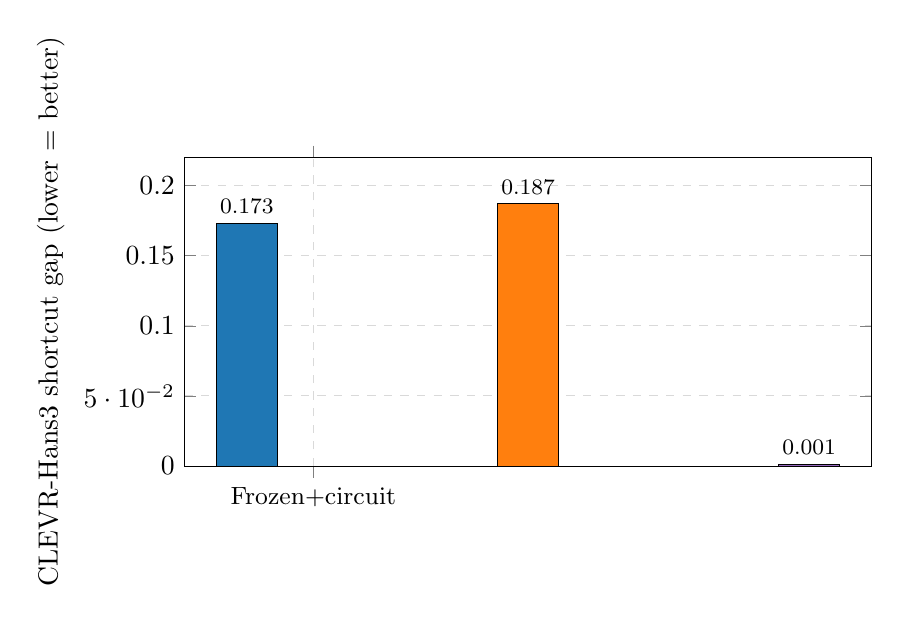
\begin{tikzpicture}
\begin{axis}[
    ybar,
    width=0.85\textwidth,
    height=5.5cm,
    bar width=22pt,
    enlarge x limits=0.30,
    ylabel={CLEVR-Hans3 shortcut gap (lower = better)},
    ymin=0, ymax=0.22,
    symbolic x coords={Frozen+circuit, Frozen+MLP, Oracle+circuit},
    xtick=data,
    xticklabel style={font=\small},
    nodes near coords,
    nodes near coords style={font=\footnotesize, /pgf/number format/.cd, fixed, precision=3},
    grid=major,
    grid style={dashed, gray!30},
]
\addplot[fill=circuitblue] coordinates {(Frozen+circuit, 0.173)};
\addplot[fill=mlporange]   coordinates {(Frozen+MLP, 0.187)};
\addplot[fill=oraclepurple] coordinates {(Oracle+circuit, 0.001)};
\end{axis}
\end{tikzpicture}
\caption{CLEVR-Hans3 shortcut gap by configuration. With frozen ResNet50 perception, circuit and MLP collapse equally (paired permutation test: $p{=}0.375$). With ground-truth scene graphs (oracle), the same reasoning head reaches a $0.001$ gap --- a $172\times$ reduction --- demonstrating that the bottleneck is upstream of the reasoning head.}
\label{fig:clevr_bar}
\end{figure}

\paragraph{Three configurations.}
\textbf{Rows 1--2 (ResNet50 frozen).} Each $224 \times 224$ RGB input image is passed through ResNet50 pretrained on ImageNet, with all weights frozen. We take the activations of the penultimate layer (after the final global-average-pool, before the $1000$-way classifier), giving a $2048$-dimensional feature vector per image. This vector is fed to a small reasoning head: either the circuit (operating as a $17$-bit-style reasoning module after linear projection to its input width), or a parameter-matched MLP. The classifier head outputs $3$ class logits via a final linear layer. Only the reasoning head and the projection are trained. This setup --- known as a \emph{concept bottleneck} in the neuro-symbolic literature --- is the standard configuration for evaluating reasoning heads on perceptual benchmarks.

\textbf{Row 3 (oracle: scene graph input).} CLEVR-Hans3 ships, alongside each rendered image, the underlying scene graph used by the rendering engine. This is a structured vector encoding every object in the scene: a sequence of $(\text{shape}, \text{color}, \text{material}, \text{size}, x, y, z)$ tuples (with shape/color/material/size one-hot encoded, and position as $\R^3$ coordinates), padded to a maximum object count. We feed this scene-graph vector directly to the same circuit reasoning head, bypassing the ResNet entirely. This row is the \emph{oracle}: it asks how well the circuit reasons \emph{given} a perfect perception front-end, isolating the contribution of the reasoning head from the contribution of the perception.

\paragraph{Statistical test.}
A paired permutation test on the circuit-vs-MLP shortcut-gap difference ($B = 10000$ flips, two-sided) gives $p = 0.375$.
The numerical 1.4 percentage point advantage for the circuit is within seed noise, and we treat it as null.
The circuit does not beat the MLP on this benchmark.

\paragraph{The oracle dissociation.}
The contrast between the frozen-ResNet rows and the oracle row is the clean signal.
With frozen ImageNet features both reasoning heads collapse to a $\sim 17$\,pt shortcut gap; with scene-graph input the same circuit reaches a $0.001$ gap --- a 172-fold reduction.
This is a clean experimental separation of two failure modes that are usually confounded in concept-bottleneck experiments:
\begin{itemize}
  \item ``The reasoning head cannot represent the rule.'' Refuted: the circuit-on-scene-graphs configuration reaches 99.9\% on the confounded validation and 99.9\% on the clean test, so the rule is representable by the same circuit architecture that fails when given ResNet features.
  \item ``The perception pipeline forwards the confound.'' Supported: frozen ImageNet features contain enough information about the spurious gray-cube correlate that any downstream head we tested (circuit or MLP) will use it.
\end{itemize}
The practical implication is that any neuro-symbolic effort to defeat CLEVR-Hans-style confounds with a frozen pretrained backbone is fighting a fight whose outcome is already determined upstream of the reasoning head.
Future work should fine-tune the perception backbone or use concept supervision to make the perceptual code informative about the true rule and uninformative about the confound.

% ============================================================================
\section{Summary of Empirical Claims}
\label{sec:claims}

\begin{table}[H]
\centering
\caption{Summary of empirical claims and their status at $n{=}5$ seeds (E4 Monks: $n{=}3$).}
\label{tab:claims}
\renewcommand{\arraystretch}{1.15}
\begin{tabular}{p{0.56\textwidth}p{0.38\textwidth}}
\toprule
\textbf{Claim} & \textbf{Status} \\
\midrule
Hard-extraction $\Delta \approx 0$ (faithfulness)                               & \textcolor{xgbgreen}{\textbf{Supported}} across E1, E3 \\
Circuit recovers Monks-1, Monks-2, Monks-3 ground-truth rules                   & \textcolor{xgbgreen}{\textbf{Supported}}, $\geq 96.5\%$ enumeration accuracy \\
Circuit exactly recovers Monks-2 counting constraint where XGBoost cannot       & \textcolor{xgbgreen}{\textbf{Supported}}, 3/3 seeds exact \\
Circuit beats MLP-matched on accuracy                                           & \textcolor{red!75!black}{\textbf{Refuted}} (parity or within noise) \\
Circuit has low-data inductive-bias advantage                                   & \textcolor{red!75!black}{\textbf{Refuted}} on 11-bit MUX \\
Circuit reduces CLEVR-Hans3 shortcut gap vs MLP-matched                          & \textcolor{red!75!black}{\textbf{Refuted}} ($p = 0.375$) \\
Reasoning head recovers true rules given good perception                        & \textcolor{xgbgreen}{\textbf{Supported}}, oracle $0.999 \pm 0.001$ \\
Frozen ImageNet perception is the bottleneck for visual shortcut resistance    & \textcolor{xgbgreen}{\textbf{Supported}} by the $172\times$ oracle/ResNet gap differential \\
\bottomrule
\end{tabular}
\end{table}

% ============================================================================
\section{What This Contributes}
\label{sec:contributions}

A genuinely modest contribution, stated cleanly.

\paragraph{A faithfulness probe protocol.}
The band-checkpoint methodology of E1/E3 (Figure~\ref{fig:band}) --- stop training at a target accuracy band, then measure hard-extraction $\Delta$ --- gives non-tautological evidence for symbolic readout faithfulness.
Standard reports of $\Delta$ at $>99\%$ accuracy are uninformative because the soft mixture has already collapsed to discrete; the band protocol forces evaluation in the regime where the question is non-trivial.

\paragraph{A clean counting-constraint result.}
Monks-2 exact recovery by all seeds while XGBoost fails by 22 points is, to our knowledge, the cleanest direct demonstration that a differentiable architecture can outperform a tree ensemble on a structurally specific reasoning task without losing tabular competence on Monks-1 and Monks-3.

\paragraph{A locating-the-failure result on CLEVR-Hans3.}
The $172\times$ gap differential between oracle and frozen-ResNet pipelines (Figure~\ref{fig:clevr_bar}) is a clean experimental separation of ``the reasoning head can do this'' from ``the perception pipeline forwards the confound.''
Future work targeting visual shortcut resistance with neuro-symbolic architectures should not freeze the perception backbone.

% ============================================================================
\section{Limitations and What Does Not Work}
\label{sec:limitations}

\begin{itemize}
  \item The circuit offers \textbf{no measurable accuracy advantage} over a parameter-matched two-layer MLP on any benchmark we tested.
  \item The circuit offers \textbf{no low-data advantage} on 11-bit MUX learning curves.
  \item The circuit offers \textbf{no visual shortcut-resistance advantage} with a frozen pretrained backbone.
  \item Multi-seed counts are $n{=}5$ for E1/E3/E5 and $n{=}3$ for E4 Monks; the CLEVR-Hans3 permutation test's negative result is therefore consistent with a true gap up to ${\sim}5$\,pt being missed.
  \item All training runs are short (band-checkpointed or capped). Full-convergence behavior may differ.
  \item The symbolic readout produced by hard extraction is a flat per-slot expression: a list of $L \times C = 64$ slot expressions, each naming an operator from the alphabet and its two input channel indices. We did not evaluate human-readability of the extracted expressions, nor attempt expression simplification (subexpression elimination, algebraic identities) that would be needed to compress this into a form a domain expert could audit at a glance.
\end{itemize}

% ============================================================================
\section{Related Work}
\label{sec:related}

The architectural lineage is \citet{petersen2022deep} (Deep Differentiable Logic Gate Networks, NeurIPS 2022) and \citet{petersen2024convolutional} (Convolutional Differentiable Logic Gate Networks, NeurIPS 2024 Oral), which achieve 86.3\% CIFAR-10 with 61M discrete-gate parameters.
Our circuit is in the same family but with a wider operator alphabet (logic $\cup$ bounded arithmetic) and is not optimized for image-classification competitiveness; the E1 numbers above are decisively below Petersen.

The neuro-symbolic / rule-extraction context includes Inductive Logic Programming (Aleph, Metagol) and Logic Tensor Networks~\citep{badreddine2021logic}, which we did not directly compare against.
The Monks suite is from~\citet{thrun1991monks}; CLEVR-Hans3 is~\citet{stammer2021right} and the published competitor we did not attempt to reproduce is the Neuro-Symbolic Concept Learner~\citep{mao2019neuro}.
Local attribution methods (LIME~\citep{ribeiro2016should}, SHAP~\citep{lundberg2017unified}, Integrated Gradients~\citep{sundararajan2017axiomatic}) are used as auxiliary diagnostics in E3.

% ============================================================================
\section{Reproducibility}
\label{sec:repro}

Every experiment in this paper is fully specified by the protocol in Section~\ref{sec:protocol} and the per-experiment details in Sections~\ref{sec:e1}--\ref{sec:e5}.
The only inputs needed to reproduce the numbers are: the random seed set $\{0, 1, 2, 3, 4\}$ (E1/E3/E5) or $\{0, 1, 2\}$ (E4); the dataset specifications (MNIST and CIFAR-10 from their canonical sources; the Monks-1/2/3 splits from~\citet{thrun1991monks}; the CLEVR-Hans3 splits from~\citet{stammer2021right}; synthetic boolean tasks generated from the closed-form definitions in Section~\ref{sec:e3}); and the architecture/optimizer settings in Tables~\ref{tab:hyper}, the protocol section, and the per-experiment configuration text.
The band-checkpoint protocol (Figure~\ref{fig:band}) is implemented as an end-of-epoch callback that snapshots model weights and triggers extraction when the validation-accuracy condition is first satisfied; this single piece of stateful logic is the only non-obvious implementation detail.

Training wall-clocks on an RTX 4090 are: E1 $<\!4$\,min/seed/dataset, E3 $<\!6$\,min/seed for all three tasks, E4 $<\!2$\,min/seed for all three Monks problems, E5 $<\!12$\,min/seed for all three configurations, for a total of approximately $50$\,min for one full $n = 5$ sweep over E1+E3+E5.

% ============================================================================
\section{Conclusion}
\label{sec:conclusion}

\circuit{} is a faithful differentiable reasoning head.
Its symbolic readout is bit-exactly what the trained model computes, robustly across seeds and tasks.
It recovers published ground-truth boolean rules from real UCI data at parity with a parameter-matched MLP, and decisively beats gradient boosting on the one Monks task whose true rule is a counting constraint.
It does not, in our hands, confer any accuracy, low-data, or visual-shortcut-resistance advantage.
The most useful follow-ups are (a) end-to-end training with concept supervision on a CLEVR-style benchmark, where the oracle-vs-ResNet result suggests there is real room to move; (b) head-to-head comparison against ILP systems on Monks-2-style structural tasks, where the circuit's exact-recovery result is most likely to remain distinctive.

% ============================================================================
\bibliographystyle{plainnat}

\begin{thebibliography}{99}

\bibitem[Badreddine et al.(2021)]{badreddine2021logic}
Badreddine, S., d'Avila Garcez, A., Serafini, L., \& Spranger, M. (2021).
\newblock Logic tensor networks.
\newblock \emph{Artificial Intelligence}, 303, 103649.

\bibitem[Lundberg \& Lee(2017)]{lundberg2017unified}
Lundberg, S.~M. \& Lee, S.-I. (2017).
\newblock A unified approach to interpreting model predictions.
\newblock \emph{Advances in Neural Information Processing Systems}, 30.

\bibitem[Mao et al.(2019)]{mao2019neuro}
Mao, J., Gan, C., Kohli, P., Tenenbaum, J.~B., \& Wu, J. (2019).
\newblock The neuro-symbolic concept learner: Interpreting scenes, words, and sentences from natural supervision.
\newblock \emph{International Conference on Learning Representations}.

\bibitem[Petersen et al.(2022)]{petersen2022deep}
Petersen, F., Borgelt, C., Kuehne, H., \& Deussen, O. (2022).
\newblock Deep differentiable logic gate networks.
\newblock \emph{Advances in Neural Information Processing Systems}, 35.

\bibitem[Petersen et al.(2024)]{petersen2024convolutional}
Petersen, F., Kuehne, H., Borgelt, C., Welzel, J., \& Ermon, S. (2024).
\newblock Convolutional differentiable logic gate networks.
\newblock \emph{Advances in Neural Information Processing Systems}, 37.

\bibitem[Ribeiro et al.(2016)]{ribeiro2016should}
Ribeiro, M.~T., Singh, S., \& Guestrin, C. (2016).
\newblock ``{Why} should {I} trust you?'': Explaining the predictions of any classifier.
\newblock \emph{ACM SIGKDD International Conference on Knowledge Discovery and Data Mining}, 1135--1144.

\bibitem[Stammer et al.(2021)]{stammer2021right}
Stammer, W., Schramowski, P., \& Kersting, K. (2021).
\newblock Right for the right concept: Revising neuro-symbolic concepts by interacting with their explanations.
\newblock \emph{IEEE/CVF Conference on Computer Vision and Pattern Recognition}, 3619--3629.

\bibitem[Sundararajan et al.(2017)]{sundararajan2017axiomatic}
Sundararajan, M., Taly, A., \& Yan, Q. (2017).
\newblock Axiomatic attribution for deep networks.
\newblock \emph{International Conference on Machine Learning}, 3319--3328.

\bibitem[Thrun et al.(1991)]{thrun1991monks}
Thrun, S., Bala, J., Bloedorn, E., Bratko, I., Cestnik, B., Cheng, J., et al. (1991).
\newblock The {MONK}'s problems: A performance comparison of different learning algorithms.
\newblock \emph{Technical Report CMU-CS-91-197}, Carnegie Mellon University.

\end{thebibliography}

\end{document}
